\documentclass[11pt,leqno]{amsart}
\usepackage[utf8]{inputenc}
\usepackage[dvipsnames]{xcolor}
\usepackage{tikz}
\usepackage{pgfplots}
\pgfplotsset{compat=newest}
\usepgfplotslibrary{fillbetween}
\usetikzlibrary{patterns}
\usepackage{color}
\usepackage{pgfplots}

\newcommand{\mf}{\mathbf}

\begin{document}

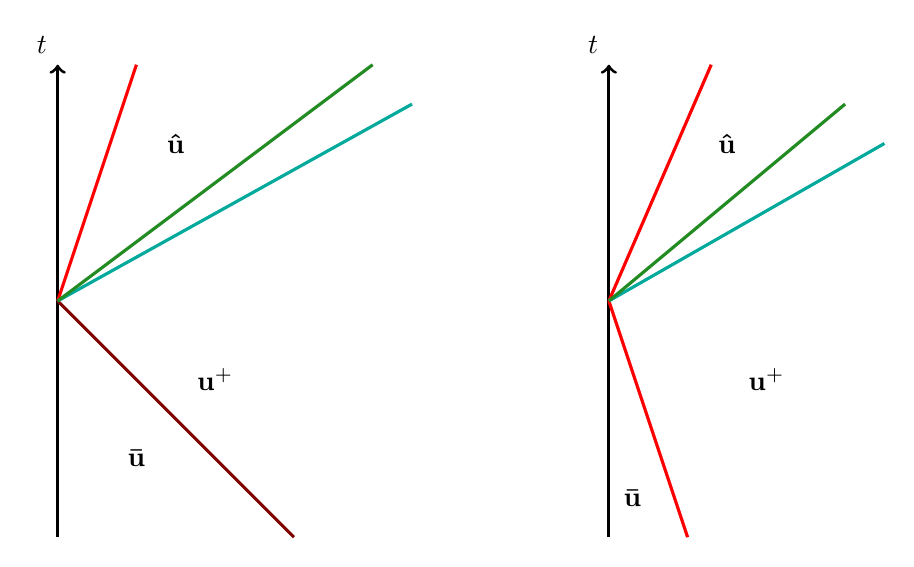
\begin{tikzpicture}
\draw[line width=0.4mm,->] (0,0) -- (0,6) node[anchor=south east] {$t$};
\draw[line width=0.4mm,Maroon]   (3, 0) -- (0, 3); 
\draw[line width=0.4mm,red]   (0, 3) -- (1, 6); 
\draw[line width=0.4mm,JungleGreen]   (0, 3) -- (4.5, 5.5); 
\draw[line width=0.4mm,ForestGreen]   (0, 3) -- (4, 6); 
\draw  (1,1) node {$\mf{\bar u}$};
\draw  (2,2) node {$\mf{u}^+$};
\draw  (1.5,5) node {$\mf{\hat u}$};
\draw[line width=0.4mm,->] (7,0) -- (7,6) node[anchor=south east] {$t$};
\draw[line width=0.4mm,red]   (8, 0) -- (7, 3); 
\draw[line width=0.4mm,red]   (7, 3) -- (8.3, 6); 
\draw[line width=0.4mm,JungleGreen]   (7, 3) -- (10.5, 5); 
\draw[line width=0.4mm,ForestGreen]   (7, 3) -- (10, 5.5); 
\draw  (7.3,0.5) node {$\mf{\bar u}$};
\draw  (9,2) node {$\mf{u}^+$};
\draw  (8.5,5) node {$\mf{\hat u}$};
\end{tikzpicture}

\end{document}